\documentclass[12pt]{book}

\usepackage[]{amsmath}
\usepackage[]{amsthm}
\usepackage[]{amsfonts}
\usepackage[]{amssymb}
\usepackage{blindtext}
\usepackage[a4paper, total={6in, 8in}]{geometry}
\usepackage{graphicx}
\usepackage{listings}
\usepackage{color}
\usepackage{array}

\definecolor{dkgreen}{rgb}{0,0.6,0}
\definecolor{gray}{rgb}{0.5,0.5,0.5}
\definecolor{mauve}{rgb}{0.58,0,0.82}

\pagenumbering{arabic}
\renewcommand{\chaptername}{Section}
\let\cleardoublepage\clearpage

\lstset{frame=tb,
  language=Python,
  aboveskip=3mm,
  belowskip=3mm,
  showstringspaces=false,
  columns=flexible,
  basicstyle={\small\ttfamily},
  numbers=left,
  numberstyle=\small\color{black},
  keywordstyle=\color{blue},
  commentstyle=\color{dkgreen},
  stringstyle=\color{mauve},
  breaklines=true,
  breakatwhitespace=true,
  tabsize=4
}

\title{EECS4443 review}
\author{Jerry Wu}
\date{2023-12-11}

\begin{document}
\maketitle
\tableofcontents

\chapter{Quiz answers}

\section*{Quiz 1: UI design, intro to activities, etc}

\begin{itemize}
    \item[1.] A design is efficient, if:
    \begin{itemize}
        \item[a)] it accomplishes the user's task in a satisfying way.
        \item[b)] it accomplishes the user's task.
        \item[c)] \textbf{it accomplishes the user's task without creating additional problems.}

    \end{itemize}
    \item[2.] Using auto-complete may help you satisfy which UX (user experience) design principle?
    \begin{itemize}
        \item[a)] \textbf{Minimize User Input}
        \item[b)] KISS (keep it simple stupid!)
        \item[c)] Make Navigation Intuitive
    \end{itemize}
    
    \item[3.] Android Applications usually follow this architectural style:
    \begin{itemize}
        \item[a)] \textbf{MVVM (a variant of MVC)}
        \item[b)] Layered
        \item[c)] Plugin
    \end{itemize}
    
    \item[4.] A design is effective, if:
    \begin{itemize}
        \item[a)] it accomplishes the user's task without creating additional problems.
        \item[b)] it accomplishes the user's task in a satisfying way.
        \item[c)] \textbf{it accomplishes the user's task.}
    \end{itemize}
    
    \item[5.] A design is exciting, if:
    \begin{itemize}
        \item[a)] it accomplishes the user's task without creating additional problems.
        \item[b)] \textbf{it accomplishes the user's task in a satisfying way.}
        \item[c)] it accomplishes the user's task.
    \end{itemize}
    
    \item[6.] When an interface puts an interactive element in a place where another element is most commonly found in other applications, what is this UX antipattern called?
    \begin{itemize}
        \item[a)] Misdirection
        \item[b)] \textbf{Bait and Switch}
        \item[c)] Roach Motel
    \end{itemize}
    
    \item[7.] In Android, an \texttt{Activity} corresponds to:
    \begin{itemize}
        \item[a)] a transition between screens.
        \item[b)] \textbf{a screen}
        \item[c)] a use case
    \end{itemize}
    
    \item[8.] If an \texttt{Activity} has been "Destroyed",
    \begin{itemize}
        \item[a)] the \texttt{onSaveInstanceState()} method is invoked automatically, so that we can always recover the Activity.
        \item[b)] it is impossible to be recovered and has to be created again from scratch.
        \item[c)] \textbf{our code needs to explicitly call the \texttt{onSaveInstanceState()} in order to recreate the Activity for certain circumstances.}
    \end{itemize}
    
    \item[9.] When an \texttt{Activity} is Paused,
    \begin{itemize}
        \item[a)] it is completely visible to the user, but inactive.
        \item[b)] it is hidden from the user and can be destroyed by the system.
        \item[c)] \textbf{it is not in the user's main focus and may be destroyed by the system.}
    \end{itemize}
    
    \item[10.] If an \texttt{Activity} is Started,
    \begin{itemize}
        \item[a)] it is not fully created, but not yet visible to the user.
        \item[b)] \textbf{it is visible, but not yet running.}
        \item[c)] it has been created, but it is hidden from the user.
    \end{itemize}

\end{itemize}

\section*{Quiz 2: Views, layouts, etc}

\begin{itemize}
    \item[1.] If I flip the orientation of my device, when I have a \texttt{GridView},
    \begin{itemize}
        \item[a)] It will maintain the same number of rows and columns.
        \item[b)] It will maintain the same number of rows and columns, but it will stretch or screen the dimensions of the items to better fit the screen.
        \item[c)] \textbf{It will adapt the number of rows and columns to better fit the screen.}
    \end{itemize}
    
    \item[2.] A \texttt{Toast} is a popup dialog that 
    \begin{itemize}
        \item[a)] Requires a user's action to disappear
        \item[b)] Provides important feedback, like a warning or an error to a user.
        \item[c)] \textbf{Automatically disappears after some time.}
    \end{itemize}
   
    \item[3.] A layout is used \textbf{only} to
    \begin{itemize}
        \item[a)] Define all the UI elements used in an application
        \item[b)] \textbf{Define all the UI elements of an activity and how they are organized.}
        \item[c)] Define the position of UI elements when the orientation of the screen changes.
        \item[d)] All of the above
    \end{itemize}
    
    
    \item[4.] A \texttt{ListView} is used to create and present lists in an \texttt{Activity}. When the \texttt{ListView} is created and presented,
    \begin{itemize}
        \item[a)] It loads all data and create the visualizations for all list items.
        \item[b)] \textbf{It loads all data in the Adapter but creates visualizations only for the visible items.}
        \item[c)] It loads only the data that will be visible, but creates placeholder items (UI elements) for all possible data items.
    \end{itemize}
   
    \item[5.] In this layout, the elements are organized "in rows and columns".
    \begin{itemize}
        \item[a)] Linear layout
        \item[b)] Relative Layout
        \item[c)] \textbf{Grid Layout}
    \end{itemize}
    
    \item[6.] In this layout, I can assign elements a certain "weights" which defines the space they will take in the layout relative to other elements in the layout.
    \begin{itemize}
        \item[a)] \textbf{Linear layout}
        \item[b)] Relative Layout
        \item[c)] Grid Layout
    \end{itemize}
    
    \item[7.] In this layout, the elements are organized using anchors, like other elements, the parent elements, or specific positions.
    \begin{itemize}
        \item[a)] Linear layout
        \item[b)] \textbf{Relative Layout}
        \item[c)] Grid Layout
    \end{itemize}
    
    \item[8.] In the Manifest, we can declare that our application requires permission to access
    \begin{itemize}
        \item[a)] \textbf{any kind of resource external to the application, which includes Internet sources or the storage of the device.}
        \item[b)] only the external storage of our device.
        \item[c)] only data sources on the Internet.
    \end{itemize}
    
    \item[9.] What is the class that is used to as a link between the layout and the data source?
    \begin{itemize}
        \item[a)] Adapter
        \item[b)] \textbf{AdapterView}
        \item[c)] Intent
    \end{itemize}

    \item[10.] When I am using a ListView, which of the following statements is true? (only one is true)
    \begin{itemize}
        \item[a)] I can have only single line textual items.
        \item[b)] I can have both single and multiple line items, but only textual items.
        \item[c)] \textbf{I can have items that combine multiple data types, text, images, icons, action buttons, and span many lines.}
    \end{itemize}

\end{itemize}

\section*{Quiz 3: Software testing methods}

\begin{itemize}
    \item[1.] In software testing, these modules accept test data from high-level modules and pass computed data.
    \begin{itemize}
        \item[a)] \textbf{Stubs}
        \item[b)] Test cases
        \item[c)] Drivers
    \end{itemize}

    \item[2.] In this type of software testing, the system is tested in parts usually following the order of development.
    \begin{itemize}
        \item[a)] Big Bang
        \item[b)] \textbf{Incremental}
        \item[c)] Alpha testing
    \end{itemize}

    \item[3.] Which MotionEvent action is called when a second finger touches the screen?
    \begin{itemize}
        \item[a)] \texttt{ACTION\_DOWN}
        \item[b)] \textbf{ACTION\_POINTER\_DOWN}
        \item[c)] \texttt{ACTION\_MOVE}
        \item[d)] \texttt{ACTION\_POINTER\_UP}
    \end{itemize}

    \item[4.] In this type of testing, users provide feedback on an incomplete version of the system.
    \begin{itemize}
        \item[a)] \textbf{Alpha testing}
        \item[b)] Beta testing
        \item[c)] Exploratory testing
    \end{itemize}

    \item[5.] Which of the following interactions is NOT a gesture?
    \begin{itemize}
        \item[a)] Swipe
        \item[b)] Flick
        \item[c)] \textbf{Click}
    \end{itemize}

    \item[6.] How many test cases do we typically need to test a software functionality?
    \begin{itemize}
        \item[a)] A lot!
        \item[b)] Exactly three (happy path, boundary path, exceptional path)
        \item[c)] \textbf{We need one test case for each invalid and boundary value and enough test cases to cover all valid equivalence classes.}
    \end{itemize}

    \item[7.] What is considered a "gesture" in the context of Android development?
    \begin{itemize}
        \item[a)] A "digital" handshake used for electronic verifications
        \item[b)] A hand motion, like a wave, capture by the camera of a mobile device.
        \item[c)] \textbf{Any tactile, i.e., using touch, interaction with the screen of the mobile device.}
    \end{itemize}

    \item[8.] A Unistroke is
    \begin{itemize}
        \item[a)] A single straight line
        \item[b)] \textbf{A continuous single line that represents a character or another symbol.}
        \item[c)] A line to represent the number 1.
    \end{itemize}

    \item[9.] In the Espresso Testing Framework, what is an Idling Resource?
    \begin{itemize}
        \item[a)] A device resource, like CPU, memory, and disk, that does not perform any task at the moment.
        \item[b)] An activity that is not visible at the moment.
        \item[c)] \textbf{An object that represents an asynchronous task running in the background.}
    \end{itemize}

    \item[10.] A "pinching" movement on the screen requires this class to be captured.
    \begin{itemize}
        \item[a)] \texttt{GestureDetector}
        \item[b)] Either \texttt{GestureDetector} or \texttt{ScaleGestureDetector}
        \item[c)] \textbf{ScaleGestureDetector}
    \end{itemize}

\end{itemize}
\newpage
\section*{Quiz 4: Fragments, SPE, etc.}

\begin{itemize}
    \item[1.] What is the difference between profiling and monitoring?
    \begin{itemize}
        \item[a)] Profiling is static, while monitoring is dynamic.
        \item[b)] Profiling is for software, while monitoring is for hardware.
        \item[c)] \textbf{Profiling is measuring at development time, monitoring is measuring after deployment.}
        \item[d)] They are the same concept.
    \end{itemize}

    \item[2.] What class do I use to pass data between two Activities?
    \begin{itemize}
        \item[a)] \texttt{Bundle}
        \item[b)] \texttt{TouchListener}
        \item[c)] \textbf{Intent}
    \end{itemize}

    \item[3.] What can be detected by the gyroscope?
    \begin{itemize}
        \item[a)] The acceleration force
        \item[b)] \textbf{The rate of rotation.}
        \item[c)] The geomagnetic field strength
    \end{itemize}

    \item[4.] One of the goals of Software Performance Engineering is to
    \begin{itemize}
        \item[a)] Allocate more resources to the software to improve its performance.
        \item[b)] Improve the efficiency of the developers.
        \item[c)] \textbf{Reduce the maintenance costs necessary to resolve performance issues.}
    \end{itemize}

    \item[5.] How can I invoke a transition between two activities?
    \begin{itemize}
        \item[a)] \textbf{By creating an Intent object to start the new activity and pass data between the activities.}
        \item[b)] by calling \texttt{Bundle.startActivity()}
        \item[c)] by calling \texttt{Intent.startActivity()}
    \end{itemize}

    \item[6.] How can I create transitions between fragments?
    \begin{itemize}
        \item[a)] With Intents like in the Activities.
        \item[b)] By declaring the fragments as "containers" in the layout XML.
        \item[c)] \textbf{By beginning a transaction through the Fragment manage and replacing the current Fragment with another one.}
    \end{itemize}

    \item[7.] When an operation is too short, which profiling method do we prefer?
    \begin{itemize}
        \item[a)] Sampling
        \item[b)] \textbf{Instrumentation}
        \item[c)] Both are equally acceptable.
        \item[d)] None of the above
    \end{itemize}

    \item[8.] Which of the following are acceptable profiling methods? (multiple answers, wrong answers will receive -25%)
    \begin{itemize}
        \item[a)] Basic profiling
        \item[b)] \textbf{Sampling}
        \item[c)] \textbf{Instrumentation}
        \item[d)] Hybrid
    \end{itemize}

    \item[9.] What is a fragment?
    \begin{itemize}
        \item[a)] \textbf{a "sub-activity"}
        \item[b)] a popup dialog
        \item[c)] a simple UI element like a menu
    \end{itemize}

    \item[10.] Why do we say that the performance being perceived by the users is a limitation of Software Performance Engineering?
    \begin{itemize}
        \item[a)] \textbf{Because during development we cannot test the performance in the same conditions, same environment and under the exact same scenarios as the users.}
        \item[b)] Because users cannot provide technical feedback about the performance of the software.
        \item[c)] Because users are not involved in the development of the software when performance requirements are implemented.
    \end{itemize}

\end{itemize}

\chapter{Sample final exam solutions}
\section*{Multiple choice questions}

\begin{itemize}
    \item[1.] In the manifest of an Android application, among other things, we specify
    \begin{itemize}
        \item[a)] \textbf{the activities of the application.}
        \item[b)] the UI elements of the application.
        \item[c)] the string constants used in our code.
    \end{itemize}

    \item[2.] When an Activity is Paused
    \begin{itemize}
        \item[a)] it is hidden from the user and can be destroyed by the system.
        \item[b)] \textbf{it is not in the user's main focus and may be destroyed by the system.}
        \item[c)] it is completely visible to the user, but inactive.
    \end{itemize} 

    \item[3.] When an interface puts an interactive element in a place where another element is most commonly found in other applications, what is this UX antipattern called?
    \begin{itemize}
        \item[a)] Misdirection
        \item[b)] \textbf{Bait and Switch}
        \item[c)] Roach Motel
    \end{itemize} 

    \item[4.] In the XML file of a layout, we typically include
    \begin{itemize}
        \item[a)] The dependencies of our app
        \item[b)] The activities of our app
        \item[c)] \textbf{The elements of an activity and their attributes}
    \end{itemize} 

    \item[5.] Which of the following UI elements allow me to make a single choice in the presence of multiple options.
    \begin{itemize}
        \item[a)] Spinners and Action Buttons
        \item[b)] Radio buttons and Checkboxes
        \item[c)] \textbf{Spinners and Radio buttons}
    \end{itemize} 
    \item[6.] In the Espresso Testing Framework, a ViewMatcher allows me to
    \begin{itemize}
        \item[a)] \textbf{Find a view and focus on it.}
        \item[b)] Perform an action on a view.
        \item[c)] Test the value of a property or data of a view.
    \end{itemize} 

    \item[7.] In this layout, the elements are organized "one after the other".
    \begin{itemize}
        \item[a)] \textbf{Linear layout}
        \item[b)] Relative Layout
        \item[c)] Grid Layout
    \end{itemize} 

    \item[8.] In this type of software testing, the system is tested in parts usually following the order of development
    \begin{itemize}
        \item[a)] Big Bang
        \item[b)] \textbf{Incremental}
        \item[c)] Alpha testing
    \end{itemize} 

    \item[9.] What is considered a "gesture" in the context of Android development?
    \begin{itemize}
        \item[a)] A "digital" handshake used for electronic verifications.
        \item[b)] A hand motion, like a wave, capture by the camera of a mobile device.
        \item[c)] \textbf{Any tactile, i.e., using touch, interaction with the screen of the mobile device.}
    \end{itemize} 

    \item[10.] This type of performance test allows us to test the behavior of the system for a given and expected workload.
    \begin{itemize}
        \item[a)] Capacity testing
        \item[b)] \textbf{Load testing}
        \item[c)] Endurance testing
    \end{itemize} 

\end{itemize}
\chapter{UI Design problems}
\newpage
\section*{Problem 1}

You are given the UI of an activity. In the picture of the UI, there are 5 design or UX problems. Point them out, explain why they are a problem and propose a solution to fix each problem. (10 points) 
\textit{Note: Some problems can be found multiple times. You need to identify 5 different problems.}

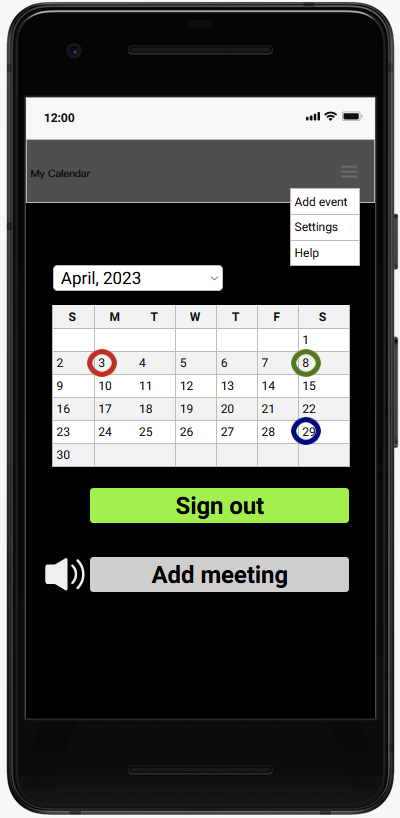
\includegraphics[scale=0.6]{images/activity.png}

\section*{Solution}
We will make a list of possible UI design issues for this activity:

\begin{itemize}
    \item The font for the title text at the top of the screen "My Calendar" is too small, so it is hard for the user to see which activity we are in. Therefore we should increase the size of the title font.
    \item The "add event" option in the spinner context menu is an important action for this activity, so it should not be in the context menu in the menu bar. We should put the action as a button under the calendar to fix this.
    \item There is no indication as to what the colours of the circle on the calendar mean. We can combat this issue by adding a legend telling us what each colour means.
    \item The action bar's colour is way too dark and it is hard to tell that it is the action bar; it isn't distinguishable. We can change this by making it a brighter colour.
    \item The "sign out" button is in a prominent position on the screen (under the calendar) when it isn't at all relevant to what the activity is supposed to do (likely adding events to a calendar). Not only that, but it is a different colour from the rest of the buttons and UI elements on the screen currently. Therefore we should get rid of it from the bottom of the screen and put it in the action bar's context menu.
    \item There is a volume icon beside "add meeting" which makes no sense. Therefore we should change the icon to something better like a "+" symbol.
\end{itemize}


\section*{Problem 2}
You are designing an assembly service for IKEA. The service allows users to input the pieces of furniture they want assembled and get a quote. The basic cost for any assembly is \$15 per item. Other factors include:
\begin{itemize}
    \item[a.] Type of furniture: Beds, cabinets, drawers (+\$10 per item); Desks, dining sets (+\$5 per item); Bookcases, chairs (basic price) 
    \item[b.] Time of assembly: Morning (basic cost), Afternoon (+\$20 for entire assembly) 
    \item[c.] Additional hourly rate: 0-3 hours (basic cost), any additional hour up to 6 hours (+\$10 per additional hour beyond 3 and until 6)
\end{itemize}
Provide the equivalence classes and the test cases for this use case. (10 points)
NOTE: \textit{You do not have to accurately calculate the result of the price for every test case.}

\section*{Solution}

We have 3 variables. 


There are \begin{itemize}
    \item 3 valid classes for type of furniture
    \item 2 valid classes for time of assembly
    \item 2 valid classes for hourly rate
\end{itemize}

There is at least one invalid class per variable (any other type of furniture, any other time of assembly and additional hours out of bounds). \\There are also four marginal values for hourly rate

\begin{itemize}
    \item 0
    \item 3
    \item 3.1
    \item 6
\end{itemize}

There must be at least 3 test cases for valid values, 4 test cases for marginal values and 3 test cases for invalid values. \textit{Deduct -1 for every test case missing (max -3 points). Do not deduct two points if it is missing both the value and the test case.}

\chapter{Prototyping problem}
You are designing “PetGPS”, a mobile app to complement a wearable digital collar for pets. The collar emits a geolocation signal captured by the app.
In the app, the user can register up to 5 collars to track different pets. The user can track the pets on a map. The user can interact with the map (zoom in and out, tap on the pet's location to see more information about the specific pet). If a pet is further than 10 meters away from where the phone with the app is, a proximity alarm goes off in the app. The app can also be connected with an autofeeder and let you know when it's time to order more food. This can be done from the pet's profile that contains information about the pet, including a picture of the pet, and gets data from the autofeeder. The user can place an order directly from the app, specifying the quantity and the type of the pet food and paying by credit card (which is already saved in the phone). Finally, the user should create a profile associated with the app and get a personalized page where they can see all their registered pets.  (30 points total)\\

Read the description carefully and answer the following questions as best and as complete as you can:

\begin{itemize}
    \item[a.] What would you include in the manifest of this app? Mention activities, permissions, intent-filters and anything else you deem relevant. (10 points)
    
    \subsection*{Solution}

    The following is a list of things included in the manifest for the app:
    \begin{itemize}
        \item[A.] \textbf{Activities}
        \begin{itemize}
            \item[1.] \texttt{UserProfileActivity}
            \item[2.] \texttt{PetProfileActivity}
            \item[3.] \texttt{MapActivity}
            \item[4.] \texttt{OrderFoodActivity}
            \item[5.] \texttt{CreateProfileActivity}
        \end{itemize}
        \item[B.] \textbf{Intent filters for activities}
        \begin{itemize}
            \item[1.] \texttt{UserProfileActivity} $\rightarrow$ \texttt{PetProfileActivity}
            \item[2.] \texttt{PetProfileActivity} $\rightarrow$ \texttt{OrderFoodActivity}
            \item[3.] \texttt{CreateProfileActivity} $\rightarrow$ \texttt{UserProfileActivity}
            \item[4.] \texttt{PetProfileActivity} $\rightarrow$ \texttt{MapActivity}
        \end{itemize}

        \item[C.] \textbf{Permissions}
        \begin{itemize}
            \item[1.] Internet for ordering food online
            \item[2.] Google services for Google maps
            \item[3.] Local storage access for pet photos
            \item[4.] GPS for location services
        \end{itemize}
    \end{itemize}


    \item[b.] What kind of listeners or other helper classes do your activities need to implement to allow for the intended interactions between the user and the app? (5 points)
    
    \subsection*{Solution}
    We can make a list of classes that we would use to implement the application's features:

    \begin{itemize}
        \item[1.] \texttt{OnTouchListener} for touch interaction with on screen lists
        \item[2.] \texttt{ScaleGestureDetector} for zooming in and out of the map
        \item[3.] \texttt{OnClickListener} for checking regular button clicks
        \item[4.] \texttt{Adapter} for handling list items
    \end{itemize}
    

    \item[c.] Provide two UI mockups, one for the user's profile and another for the pet's profile. What kind of UI elements would you choose? What kind of Layouts would you use for the two activities? (10 points)
    
    \subsection*{Solution}

    Let us list out all the UI elements we will use for both activities

    \begin{itemize}
        \item[A.] \textbf{User profile}
        \begin{itemize}
            \item List of pets
            \item Button for adding a new pet
            \item Menu for editing profile
            \item Sign out button, settings button, etc.
        \end{itemize}
        \item[B.] \textbf{Pet profile}
        \begin{itemize}
            \item Activity with 2 fragments: one with photo(s) of pet and another with the pet's information under the photo. We also need buttons to open the map to locate the pet (it opens \texttt{MapActivity}) and to order food (it opens \texttt{OrderFoodActivity}).
        \end{itemize}
    \end{itemize}
    

    \item[d.] Write test case to test the use case where the user places an order for pet food after they have received a signal from the autofeeder. (5 points)
    
    \subsection*{Solution}
    We do this by listing setup, data, procedure, and expected result.

    \begin{itemize}
        \item[A.] \textbf{Setup:} \begin{itemize}
            \item[1.] Food alarm has gone off
            \item[2.] User opens \texttt{OrderFoodActivity} for one of their pets
        \end{itemize}

        \item[B.] \textbf{Data:} \begin{itemize}
            \item Pet's name is Lucy
            \item Past order is "\date{2023-02-15}, 7kg dry food"
            \item Order was fulfilled by PetSmart (URL)
        \end{itemize}

        \item[C.] \textbf{Procedure:} \begin{itemize}
            \item[1.] User clicks on renew order
            \item[2.] User clicks on confirm new order
            \item[3.] User clicks pay button to pay for order
            \item[4.] User confirms payment for stored payment method (credit card)
        \end{itemize}

        \item[D.] \textbf{Expected result:} \begin{itemize}
            \item[1.] Confirmation toast shows up to alert the user that payment was confirmed
            \item[2.] Data about last order is updated in pet's profile
            \item[3.] Order status is set to "pending"
        \end{itemize} 
    \end{itemize}


\end{itemize}

\chapter{Constructing equivalence class tables}
To construct this table, we need the following columns:

\begin{itemize}
    \item Variable
    \item Valid class
    \item Valid value
    \item Boundary value
    \item Invalid class
    \item Invalid value
\end{itemize}

The minimum number of test cases is calculated with the following formula:

\begin{align*}
    N_{cases}=max\{N_{vals,valid}\}+max\{N_{vals,boundary}\} + N_{vals,invalid}
\end{align*}

\includegraphics*[scale=0.4]{images/equivtable.jpg}
In this chart:

\begin{itemize}
    \item The valid class with most valid values would be age. So $Max\{N_{vals,valid}\}=3$ since we take 8.4, 42.7, and 65
    \item We can use age's boundary values as well since we want the one with the most values. Therefore $Max\{N_{vals,boundary}\}=6$
    \item Finally, $N_{vals,invalid}=6$
\end{itemize}

All in all, 3+6+9=15, so we have that the minimum number of test cases for this set of specifications would be 15.

\includegraphics*[scale=0.35]{images/testtable.jpg}
Here is the chart detailing each of the test case.

\chapter{Extra quiz questions}

\end{document}